\chapter{Results}
\label{chap:results}

In this chapter we present results from the evaluation phase.

\section{Testing environment}
Access was given to a dedicated server in order achieve more control of the environment so as to get more dependable measurements. However, it should emphasized that the the purpose of doing the measurements was not to perform an experiment and we do not claim to have done so. Instead, the goal was to assess initial feasibility of the solutions and see if they would perform in an adequate manner. More specifically, we ask if the measurements of disk usage, memory utilization, insertion time, query response time etc.\ are good enough to warrant going forward beyond prototype construction.

Some notable specs on the dedicated server; \\
Operating system: Redhat Linux 6.6 \\
Processor: Intel Xeon 48 cores \\
RAM: 256 GB \\
Storage: 2TB


\section{Data separation}
For evaluation and testing purposes, access was given to a CIMS instance with a database containing about 2 years worth of data (see figure~\ref{fig:jeTrend}), where the job event table contains about 480 million rows. This is the largest database with real data that could be safely accessed for evaluation purposes, without disturbing the production environment. Using the developed software components for transforming and migrating data, all relevant data from the CIMS instance was moved to the databases of the archive prototypes. Some measurements were done during the migration process, specifically how much time the process took. This was done mainly to get ball park figures to answer if the expected time is likely to be hours, days or weeks.     
 

\section{Query support}

The set of important queries defined in section~\ref{sec:usecases} has been implemented for the archive prototypes using mongodb and elasticsearch. This section describes the outcome of this implementation and reasoning about the complexity of the queries.  

Implementation of all important queries was successful, as can be seen in section~\ref{sec:archiveapi}. How the queries for the archive is written and the effectiveness of the queries is highly dependent on the design of the non relational schema described in section~\ref{nosqlmodel}. Several differences in query properties of the prototypes compared to the CIMS database has been noted. Due to the denormalization of data, fewer joins are required for the non-relational databases and the joins that are performed are done on the application level. Joins on this level leads to more round trips to the database, but lightens the computational resources used by the database.

\hiddensubsection{Elasticsearch}


\hiddensubsection{MongoDB}

Vad skiljer sig mysql queriesen mot nosql:
    * Joins görs på applikationsnivå
    * Mer roundtrips
    * Index på allt (es)
    * Ad hoc queries (es)
    * Fri text sök, could enable better data analysis (es)

%\begin{table}[h]
%\begin{tabular}{|l|l|l|}
%\hline
%\textbf{High level query}                & \textbf{Supported} & \textbf{Comment}           \\ \hline
%Get build                                    & Y                                                                                        &                            \\ \hline
%Get build information                        & Y                                                                                        &                            \\ \hline
%Get build for root test suite                & Y                                                                                        &                            \\ \hline
%Get trouble reports for build                & Y                                                                                        &                            \\ \hline
%Get trouble report fixes for build           & Y                                                                                        &                            \\ \hline
%Get trouble reports for product and revision & Y                                                                                        &                            \\ \hline
%Get test suite children                      & Y                                                                                        &                            \\ \hline
%Get test case in build                       & Y                                                                                        &                            \\ \hline
%Get test suite in build                      & Y                                                                                        &                            \\ \hline
%Get root test suite for test case/test suite & Y                                                                                        &                            \\ \hline
%Get test case by name                        & Y                                                                                        & Used for test case history \\ \hline
%Get test suite for test case                 & Y                                                                                        &                            \\ \hline
%Get test case history                        & P                                                                                        & Tags not supported         \\ \hline
%Get test tree                                & P                                                                                        & Runs slow for large trees  \\ \hline
%\end{tabular}
%\caption{Possible values in the supported column are yes/no/partially.}
%\label{tab:archivequeries}
%\end{table}

%\section{Schema evolution}
%Not yet addressed

\section{Scalability}
\subsection{Disk usage}
The first migration performed was that of the previously mentioned CIMS instance with 480 million rows in the job event table. Disk usage is presented in figure~\ref{fig:disc}. In order to perform larger migrations, dummy job event data was generated up to a total of 3.3 billion documents/rows and inserted into the archive databases (see figure~\ref{fig:discbig}. The reason for not going beyond 3.3 billion is simply that for the testing environment that was provided the available storage would not suffice (2TB). However, with current growth trends, 3.3 billion documents/rows would still represent several years worth of historical data.

\begin{figure}[h!]
\centering
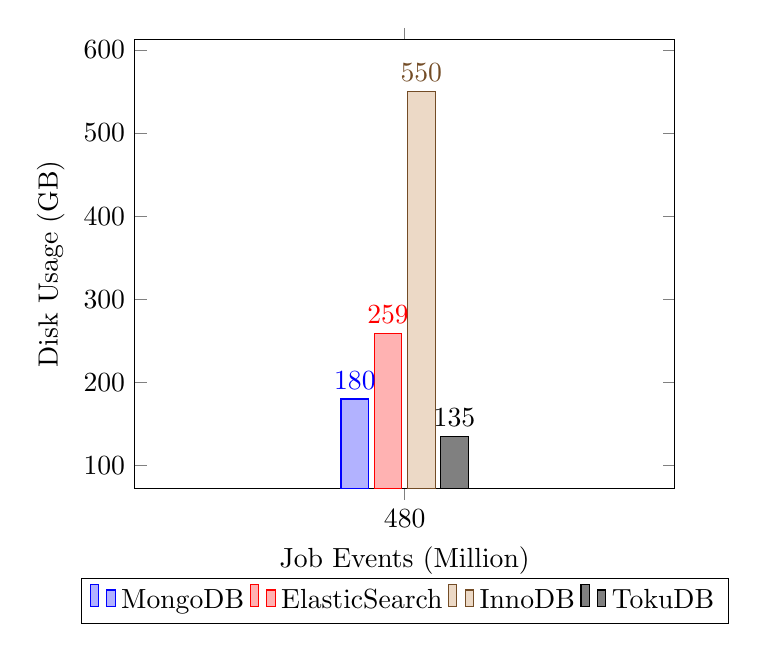
\begin{tikzpicture}
\begin{axis}[
    ybar,
    enlargelimits=0.15,
    legend style={at={(0.5,-0.2)},
      anchor=north,legend columns=-1, },
    xlabel={Job Events (Million)},
    ylabel={Disk Usage (GB)},
    symbolic x coords={480},
    xtick=data,
    nodes near coords,
    nodes near coords align={vertical},
    ]
\addplot coordinates {(480,180)};
\addplot coordinates {(480,259)};
\addplot coordinates {(480,550)};
\addplot coordinates {(480,135)};
\legend{MongoDB,ElasticSearch,InnoDB, TokuDB}
\end{axis}
\end{tikzpicture}
\caption{Disk usage after migrating data from CIMS instance with real data.}
\label{fig:disc}
\end{figure}

\begin{figure}[h!]
\centering
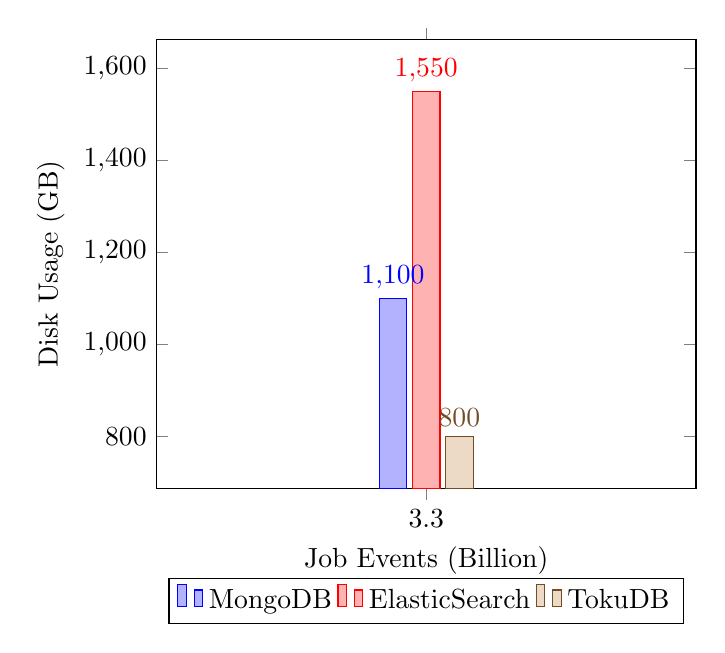
\begin{tikzpicture}
\begin{axis}[
    ybar,
    enlargelimits=0.15,
    legend style={at={(0.5,-0.2)},
      anchor=north,legend columns=-1, },
    xlabel={Job Events (Billion)},
    ylabel={Disk Usage (GB)},
    symbolic x coords={3.3},
    xtick=data,
    nodes near coords,
    nodes near coords align={vertical},
    ]
\addplot coordinates {(3.3, 1100)};
\addplot coordinates {(3.3, 1550)};
\addplot coordinates {(3.3, 800)};
\legend{MongoDB,ElasticSearch,TokuDB}
\end{axis}
\end{tikzpicture}
\caption{Disk usage after having a combination of real data and generated data.}
\label{fig:discbig}
\end{figure}

\subsection{Memory utilization}

\hiddensubsubsection{Elasticsearch}
In Elasticsearch some configuration related to memory usage is needed to achieve stable performance. It is recommended to set the JVM heap size that ES uses to no more than half of total RAM available but never no more than 32GB \cite{ESmemory}. Elasticsearch will typically use more memory than just the heap size, but this usage will be delegated to the operating system. Tests were done with 8GB, 16GB and 32GB heap size for both querying and insertion. For insertion using an 8GB heap would make Elasticsearch crash since garbage collection could not keep up. But 16 and 32GB gave stable insertion performance. However, there was no observable difference in insertion rates between 16 and 32GB heap sizes. When doing mass insertion Elasticsearch would quickly reserve half of available system memory. So insertion rates certainly seem to scale with available RAM.

On the other hand querying was different. Performing many subsequent queries would not pool RAM like insertion did. Also no positive effect on response time could be observed by increasing the heap size. Elasticsearch was stable with 8, 16 and 32 heap sizes and response times were the same.


\hiddensubsubsection{MongoDB}

Working set estimations are presented in figure~\ref{fig:ws}. Initial estimations of the working set for MongoDB have been done with manual testing. As long as custom indexes defined on the job event collection fit in RAM, the database is stable and can respond to queries where indexes can be utilized. The working set estimation is the summed size of the custom indexes. 

\begin{figure}[h!]
\centering
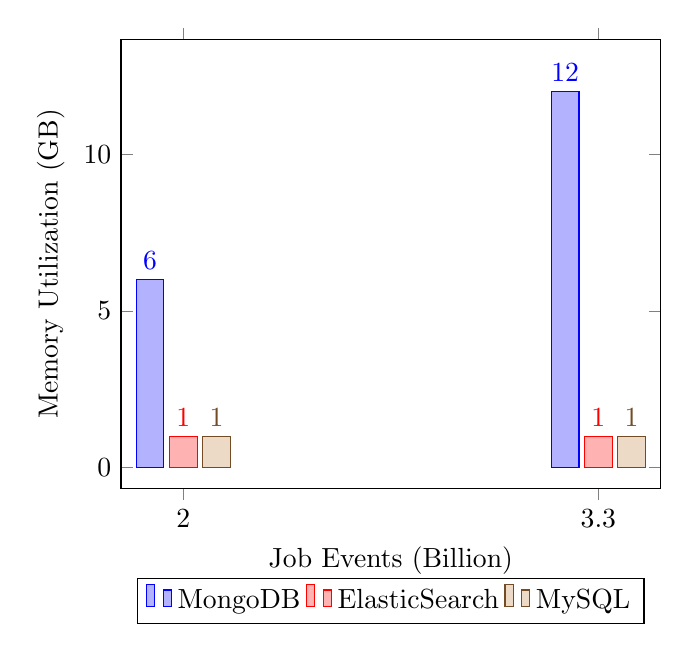
\begin{tikzpicture}
\begin{axis}[
    ybar,
    enlargelimits=0.15,
    legend style={at={(0.5,-0.2)},
      anchor=north,legend columns=-1, },
    xlabel={Job Events (Billion)},
    ylabel={Memory Utilization (GB)},
    symbolic x coords={2,3.3},
    xtick=data,
    nodes near coords,
    nodes near coords align={vertical},
    ]
\addplot coordinates {(2,6) (3.3,12)};
\addplot coordinates {(2,1) (3.3,1)};
\addplot coordinates {(2,1) (3.3,1)};
\legend{MongoDB,ElasticSearch,MySQL}
\end{axis}
\end{tikzpicture}
\caption{Working set estimation}
\label{fig:ws}
\end{figure}


\subsection{Insertion time}

\hiddensubsubsection{Elasticsearch}
We configured Elasticsearch to use a 1 node setup and migrated the CIMS instance. With this configuration the process took 21 hours. We then proceeded to insert dummy data up to a total of 3.3 billion documents. During the insertion of dummy data we could achieve a mean insertion rate of 32 million documents per hour. What is very notable here is that even using a 1 node setup we observed no performance degradation for insert rates when the total data set grew. So when going from 480 million to 3.3 billion the insert rate was as far as we could observe constant.

When switching to a 4 node setup (4 ES instances running on the same machine), much greater insert rates could be achieved and we observed over 60 million per hour in this case.

\hiddensubsubsection{MongoDB}

\hiddensubsubsection{TokuDB}


\subsection{Horizontal Scalability}
Not yet addressed
Här borde vi kunna skriva tekniska saker, men från de tekniska saker dra slutsater i Discussion som svarar på om dessa tekniker ger något business value?
\hiddensubsubsection{MongoDB}
\hiddensubsubsection{Elasticsearch}
"Lessons learned while scaling with Elasticsearch, future work can be to test with more nodes".\\
Compared to MongoDB, horizontal scaling with Elasticsearch demands more configuration upfront in order to get a suitable cluster. 
In MongoDB, where the process of adding new nodes to a cluster is not limited on how the initial node is configured, the maximum number of nodes in an Elasticsearch cluster must be known on beforehand. This restriction depends on how Elasticsearch is scaling in an horizontal manner. The partitioning of data when adding new nodes to a cluster is dependent on how many shards the initial node holds, as an new node is added to the cluster it overtakes shards from the already existing nodes.

\hiddensubsubsection{TokuDB}
\section{Organizational suitability}
This section describes the organizational suitability of the different artifacts.
\hiddensubsection{MongoDB}
\hiddensubsection{Elasticsearch}
\hiddensubsection{TokuDB}